\documentclass[11pt]{scrartcl}
\usepackage{wrapfig}
\usepackage{verbatim} 

\usepackage[T1]{fontenc} % Use 8-bit encoding that has 256 glyphs
\usepackage{fourier} % Use the Adobe Utopia font for the document - comment this line to return to the LaTeX default
%\usepackage[english]{babel} % german headers
\usepackage{ucs}             % neccessary for äöü
\usepackage[utf8x]{inputenc} % utf8 support
\usepackage{amsmath,amsfonts,amsthm} % Math packages
\usepackage{hyperref}   % use for hypertext links, including those to external documents and URLs
\usepackage{enumitem}
\usepackage{float}
\usepackage{extramarks} % Required for headers and footers
\usepackage{graphicx} % Required to insert images
\usepackage{subfigure} % Required to insert images
\usepackage{listings} % Required for insertion of code
\usepackage{courier} % Required for the courier font
\usepackage{color}
\usepackage{sectsty} % Allows customizing section commands
\usepackage{epstopdf}

\usepackage{cite}
\usepackage{textcomp}
\usepackage{subfiles}
% Style of citations
\bibliographystyle{plain}  
\usepackage{./sty/fhv}

%language
\usepackage[ngerman]{babel}


%general data
\newcommand{\myauthor}{Höss, Petrovic, Wallis}
\newcommand{\mytitle}{Dokumentation des OS}
\newcommand{\myuniversity}{Fachhochschule Vorarlberg}
\newcommand{\mycourse}{S1: Softwarelösungen für ressourcenbeschränkte Systeme}
\newcommand{\mystudy}{Master Informatik (ITM2)}
\newcommand{\mydate}{\today{}, Dornbirn}
%document meta data
\title{\mytitle}
\author{\myauthor}
\date{\today{}, Dornbirn}

%header/footer - KOMA
\usepackage{lastpage}
\usepackage[automark]{scrpage2}
\pagestyle{scrheadings}
\clearscrheadfoot
%header left
\ihead[]{\headmark}
%header center
\chead[]{}
%header right
\ohead[]{
\includegraphics[width=2cm]{figures/FHV} }
%footer left
\ifoot[]{\myauthor}
%footer center
\cfoot[]{}
%footer right
\ofoot[]{\thepage\ von \pageref{LastPage}}

\begin{document}

%%Titelseite
\begin{titlepage}

\begin{minipage}{.5\textwidth} 
  \hspace{12cm}\hfill 
\includegraphics[width=3cm]{figures/FHV} 
\end{minipage}\vspace{2cm} 

\begin{center}
~
\vfill\vfill\vfill

{\Huge\bfseries\mytitle}

\vfill

\Large{eine Arbeit von}

\vfill

{\LARGE\bfseries\myauthor}
\vfill
{\Large\bfseries\mystudy}
\vfill
\vfill
\Large{für die Lehrveranstaltung}

\vfill

{\LARGE\bfseries\mycourse}

\vfill\vfill\vfill
\vfill\vfill\vfill
\vfill\vfill\vfill

\myuniversity
\vfill
\mydate
\end{center}
\end{titlepage}
%%Ende Titelseite

%%Abstract
\begin{abstract}
\thispagestyle{plain}
	
\section*{Abstract}

\end{abstract}

\thispagestyle{plain}
%%Inhaltsverzeichnis
\tableofcontents

%%Abbildungsverzeichnis
\listoffigures

\pagebreak

\section{Allgemein}
bla

\subsection{Aufbau}
bla

\pagebreak 
\section{Architektur}
\label{chapArch}
Dieses Kapitel beschreibt die entwickelte Architektur des Betriebssystems und gibt einen groben Überblick über die einzelnen Komponenten. Detailliertere Informationen zu den einzelnen Komponenten werden in den folgenden Kapiteln beschrieben.

\subsection{Art des Kernels}
Das Betriebssystem wurde als Monolithischer Kernel umgesetzt, respektive wurden die Speicherverwaltung, Prozessverwaltung, Treiber und andere Kernelkomponenten in einem einzelnen Kernelprozess implementiert. Durch die Zusammenführung dieser Komponenten verliert das Betriebssystem zwar die Eigenschaft, nach einem Absturz einer einzelnen Komponente weiter lauffähig zu sein, allerdings darf mit diesem Konzept durchaus von einer höheren Performanz ausgegangen werden.
Ein weiterer Grund für einen Monolithischen Kernel ist das entfallen der aufwändigen Kommunikationen zwischen den verschiedenen Komponenten des Betriebssystems, welche besonders in der Anfangsphase der Entwicklungsarbeiten zu Problemen führen kann.

\subsection{Ansatz für die Abstraktionen im Betriebssystem}
Um eine möglichst gute Abstraktionen der Betriebssystem-Implementierung zu gewährleisten, wurden für die Verwaltung einzelner Kernelkomponenten \textit{Manager} verwendet. Im Allgemeinen gilt, dass die einzelnen \textit{Manager} jeweils die Schnittstelle für eine Komponente darstellen. Die Kommunikation zwischen zwei Komponenten erfolgt ausschließlich über die bereitgestellte Schnittstelle des \textit{Managers}. Eine Übersicht der einzelnen \textit{Manager} sowie eine bzw. mehrere zugehörige Funktionen, ist in Tabelle \ref{table:Manager-function} angegeben.

\begin{table}[H]
\begin{tabular}{p{4cm} | p{9cm}}
  \textbf{Managername} & \textbf{Beispiel Funktion(en)} \\ 
  \hline
  \textit{DeviceManager} & \texttt{InitDevice}, \texttt{OpenDevice}, \texttt{ReadDevice} \\
  \textit{DriverManager} & \texttt{GetDriver} \\
  \textit{FileManager} & \texttt{OpenFile}, \texttt{OpenExecutable} \\
  \textit{MemManager} & \texttt{GetFreePagesInProcessRegion}, \texttt{GetRegion} \\
  \textit{ProcessManager} & \texttt{StartProcess}, \texttt{KillProcess} \\
  \textit{IpcManager} & \texttt{RegisterNamespace}, \texttt{SendMessage} \\
 \end{tabular}
 \caption{Übersicht der Manager mit beispielhaften Funktionen}
 \label{table:Manager-function}
\end{table}

\subsection{Allgemeiner Aufbau der Architektur}
\label{section:generalArchitecture}
In Abbildung \ref{fig:general-Architecture} ist der allgemeine Aufbau mit den wesentlichen Kernelkomponenten ersichtlich. Zusätzlich zu den einzelnen Komponenten ist ebenfalls der Informationsfluss dargestellt.

\begin{figure}[H]
	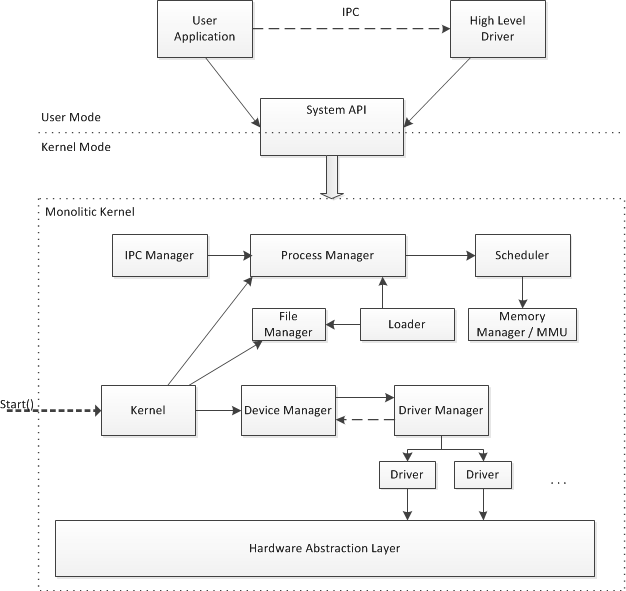
\includegraphics[scale=0.9]{chapters/architecture/figures/architecture}
	\caption{Allgemeiner Aufbau der Architektur}
	\label{fig:general-Architecture}
\end{figure}

Die oben angeführten Komponenten und deren Verantwortlichkeiten sind im Folgenden grob beschrieben: \\

\begin{description}
	\item[Hardware Abstraction Layer (HAL)] \hfill \\
	Der \ac{HAL} abstrahiert sämtlichen Hardwarezugriff des Betriebssystems und erlaubt so eine einfache Portierbarkeit auf andere Plattformen. Der Aufbau des \ac{HAL} wird in Kapitel \ref{chapHAL} beschrieben.
	
	\item[Driver] \hfill \\
	Ein Treiber bietet eine abstrakte Schnittstelle zur jeweiligen Hardware, respektive implementiert dieser die konkrete Ansteuerung. Der Aufbau der Treiber ist in Kapitel \ref{chapDriver} dokumentiert. 
	
	\item[\textit{DriverManager}] \hfill \\
	Der \textit{DriverManager} dient zur Verwaltung der Treiber, welche vom Betriebssystem zur Verfügung gestellt werden. Sollte ein Treiber benötigt werden, kann über die Schnittstelle des \textit{DriverManagers} der Zugriff auf den Treiber erfolgen. Der detaillierte Aufbau des \textit{DriverManager} ist in Kapitel \ref{secDriverManager} erläutert.
	
	\item[\textit{DeviceManager}] \hfill \\
	Der \textit{DeviceManager} ist eine weitere Abstraktion zur Verwaltung von Treibern, respektive einzelnen Geräten. So sind beispielsweise auf Treiberebene alle vier Board-LEDs als identisch anzusehen, allerdings stellen sie auf Geräteebene jeweils vier unterschiedliche Geräte dar, welche aber vom selben Treiber angesprochen werden können. In Kapitel \ref{secDeviceManager} wird die Verantwortlichkeit des \textit{DeviceManagers} genauer diskutiert.
	
	\item[Kernel] \hfill \\
	Der Kernel weist die Verantwortlichkeit für das Starten der einzelnen Komponenten auf und stellt grundlegende Funktionsschnittstellen für die einzelnen Komponenten zur Verfügung. Beispielsweise werden sämtliche Fehler oder Ausgaben von Kernelkomponenten an den Kernel selbst propagiert.
	
	\item[\textit{ProcessManager}] \hfill \\
	Der \textit{ProcessManager} stellt eine Schnittstelle für den Zugriff auf Prozesse zur Verfügung. Weiters verwaltet der \textit{ProcessManager} Meta-Daten zu den einzelnen Prozessen, wie Prozessname, Startzeit usw. Implementierungsdetails zum \textit{ProcessManager} werden in Kapitel \ref{secProcessManager} beschrieben.
	
	\item[\textit{Scheduler}] \hfill \\
	Der \textit{Scheduler} verwaltet die Prozesse auf einer abstrakten Ebene, respektive hinsichtlich ihrer Zustände, ihres Kontexts usw. Weiters ist der \textit{Scheduler}für die Umsetzung des präemptiven Multi-Taskings verantwortlich. Die konkrete Implementierung ist in Kapitel \ref{secScheduler} beschrieben.
	
	\item[\textit{MemoryManager}/\ac{MMU}] \hfill \\
	Der \textit{MemoryManager} stellt die Schnittstelle zum virtuellen Speichermanagement zur Verfügung. Diese Komponente übernimmt ebenfalls die Verwantwortlichkeit für die Verwaltung des virtuellen und physischen Speichers. Der \textit{MemoryManager} bzw. das Speichermanagement im Allgemeinen ist im Kapitel \ref{chapVirtualMemory} beschrieben.

	\item[\textit{FileManager}] \hfill \\
	Der \textit{FileManager} stellt die Schnittstelle zum Zugriff auf das Dateisystem, respektive Dateien und Ordner zur Verfügung. Der \textit{FileManager} verwaltet ebenfalls die \ac{CWD} des Benutzers bzw. der Benutzerin.
	
	\item[\textit{Loader}] \hfill \\
	Der \textit{Loader} ist für das Laden von Anwendungen verantwortlich, respektive lädt der \textit{Loader} eine Anwendung von einem externen Speichermedium in den Arbeitsspeicher, sodass dieser als Prozess ausgeführt werden kann.
	
	\item[\textit{IPCManager}] \hfill \\
	Der \textit{IPCManager} ist für die Kommunikation zwischen verschiedenen User-Anwendungen zuständig. Die Dokumentation der Interprozesskommunikation ist in Kapitel \ref{chapIPC} festgehalten.
	
	\item[System-API] \hfill \\
	Die System-API stellt eine Schnittstelle zum Betriebssystem für Anwendungen zur Verfügung. Hierdurch sind die Betriebssystemfunktionen von der Anwendung selbst entkoppelt. Dies erlaubt einen sicheren Zugriff auf Geräte und Ressourcen. Die System-API ist in Kapitel \ref{chapAPI} beschrieben.
	
	\item[\textit{User Application}] \hfill \\
	\textit{User Applications} (dt. Anwendung) sind Prozesse welche von einem externen Speichermedium geladen werden. Diese können mittels Interprozesskommunikation mit anderen Anwendungen oder mittels der System-API mit anderen Komponenten kommunizieren. Im Kapitel \ref{chapApp} ist eine konkrete Implementierung einer Anwendung dokumentiert.
	
	\item[\textit{High Level Driver}] \hfill \\
	\textit{High Level Driver} sind Treiber, welche einer Anwendung eine breitere Schnittstelle als Kernel-interne Treiber anbieten und unter anderem auch erweiterte Funktionen implementieren. Beispielswiese wird durch den \textit{High Level Driver} für das Ansteuern eines \textit{Moving Heads} über das \ac{DMX}-Protokoll das zyklische Senden des aktuellen Zustands realisiert. 
\end{description}

\pagebreak 
\section{HAL}
bla

\subsection{Aufbau}
bla

\pagebreak 
\section{Treiber}
Die Treiber stellen eine abstrakte Schnittstelle auf den Hardware Abstraction Layer dar. Dadurch muss nicht mehr direkt auf die einzelnen Hardwarekomponenten zugegriffen werden. Ein wesentlicher Aspekt bei der Architektur der Treiber war Abstraktion. Dadurch wird gewährleistet, dass jeder Treiber über die selbe Schnittstelle angesprochen werden kann. Zudem ist die Verwaltung durch den Driver Manager erleichtert.

\subsection{Aufbau eines Treibers}
In Listening \ref{generalDriverInterface} ist die allgemeine Schnittstelle für jeden Treiber ersichtlich. Jeder implementierte Treiber muss diese vorweisen können, ein Beispiel (LED Treiber) dazu ist in Listening \ref{ledDriver} zu sehen.

\lstinputlisting[language=C, caption=Allgemeine Schnittstelle für einen Treiber, label=generalDriverInterface]{chapters/driver/codefiles/generalDriverInterface.c}

\lstinputlisting[language=C, caption=Implementierung der allgemeinen Treiberschnittstelle (LED Beispiel), label=ledDriver]{chapters/driver/codefiles/ledDriver.c}


\pagebreak 
\section{Zusammenfassung und Ausblick}
\label{summary}

In diesem Kapitel werden die erreichten Ergebnisse zusammengefasst. Weiters wird ein Ausblick auf Möglichkeiten der Weiterentwicklung geboten.

\subsection{Zusammenfassung}

Das primäre Ziel dieses Projektes war die Erlangung tiefergehende Kenntnisse in Bezug auf die Systemprogrammierung von Systemen mit beschränkten Ressourcen. Dabei sollten vor allem die theoretische Grundlagen von Betriebssystemen praktisch umgesetzt werden. \\
 
Implementiert und getestet wurde ein Betriebssystem welches sich auch in Langzeittests als stabil erwiesen hat. Das Betriebssystem ist durch die HAL flexibel und ohne größere Aufwände protierbar. Zudem ist es möglich, von einer MicroSD-Karte Applikationen zu laden und auszuführen. 
Bei der Implementierung wurden sämtliche Grundaspekte moderner Betriebssysteme, wie beispielsweise die Interprozesskommunikation oder die virtuelle Speicherverwaltung, behandelt. Zudem wurden die Sicherheitsrisiken durch das saubere Trennen der Adressräume und Benutzermodi stark verringert. \\
 
Es ist zu erwähnen, dass während des Entwicklungsprozesses erwartete wie auch nichterwartete Probleme aufgetreten sind. Diese betreffen in erster Linie Komplikationen, die durch falsches Setzen der Hardwareregister entstanden sind. \\
 
Für das entworfene Betriebssystem wird kein Anspruch auf Vollständigkeit erhoben, da seine Entwicklung agil vorgenommen wurde. So wurden aus Zeitgründen bei der Erstellung der HAL nur die für die vorgesehene DMX-Applikation benötigten Funktionen implementiert. \\
 

\subsection{Ausblick}

Das Betriebssystem ist in der vorliegenden Form voll einsatzbereit und erfüllt alle gesetzten Anforderungen. Daher wird an dieser Stelle seine Entwicklung seitens des Projektteams eingestellt. Unter dem in der Einleitung angegebenen Repository auf GitHub kann es frei zugänglich heruntergeladen werden. Nachfolgend werden Ansatzpunkte für Verbesserungen bzw. Weiterentwicklungen augelistet.

\subsubsection{Punkte mit Verbesserungspotential}
Einige Punkte des Betriebssystem konnten nicht vollständig abgedeckt werden. Diese Punkte mit Verbesserungspotential werden in Tabelle \ref{table:points-to-improve} kurz beschrieben.

\begin{table}[H]
\begin{tabular}{p{5cm} | p{9cm}}
  \textbf{Sachverhalt} & \textbf{Beschreibung}
  \\ \hline
  Caching & Die aktuelle Speicherverwaltung ist ein non-caching System. Eine Einführung des Cachings für Daten hätte eine Verbesserung der Performance zur Folge. \\
  
 \end{tabular}
 \caption{Übersicht der Punkte mit Verbesserungspotential}
 \label{table:points-to-improve}
\end{table}

\subsubsection{Fehlende Punkte für eine praktische Verwendung des Betriebssystems}
Das Betriebssystem weist einige wenige Punkte auf, welche noch nicht implementiert wurden, aber für eine praktische Verwendung fehlen. Tabelle \ref{table:missing-points} zeigt diese Punkte auf.

\begin{table}[H]
\begin{tabular}{p{5cm} | p{9cm}}
  \textbf{Fehlender Punkt} & \textbf{Beschreibung}
  \\ \hline
  ResourceManager & Dieser Manager ist für die Verwaltung von Ressourcen zuständig. Dazu zählen XXX\\
  
 \end{tabular}
 \caption{Übersicht der fehlenden Punkte}
 \label{table:missing-points}
\end{table}

\clearpage
\phantomsection
\addcontentsline{toc}{chapter}{Literaturverzeichnis}
\bibliography{./bib/Bibliography}

\end{document}